\documentclass[12pt]{mwart}

\usepackage{polski}
\usepackage[utf8]{inputenc}
\usepackage{mathtools,amsthm,amssymb,icomma,upgreek,xfrac, graphicx, scrextend, float, adjustbox, nameref}
\usepackage{tabularray}
\usepackage[labelfont=bf]{caption}
\mathtoolsset{mathic}
\raggedbottom
\graphicspath{ {./images/} }

\author{Mateusz Stasiak \\ Indeks: 262339}
\title{Instrukcja tworzenia sygnału w Xcos}

\begin{document}
	\maketitle
	
	\section{Zadanie}
	\noindent Stwórz sygnał o kształcie odpowiadającym miesięcznemu wykresowi kursu rupii nepalskiej w dniach 01.05.2022 - 01.06.2022 r. 
	
	\begin{figure}[H]
	\begin{center}
		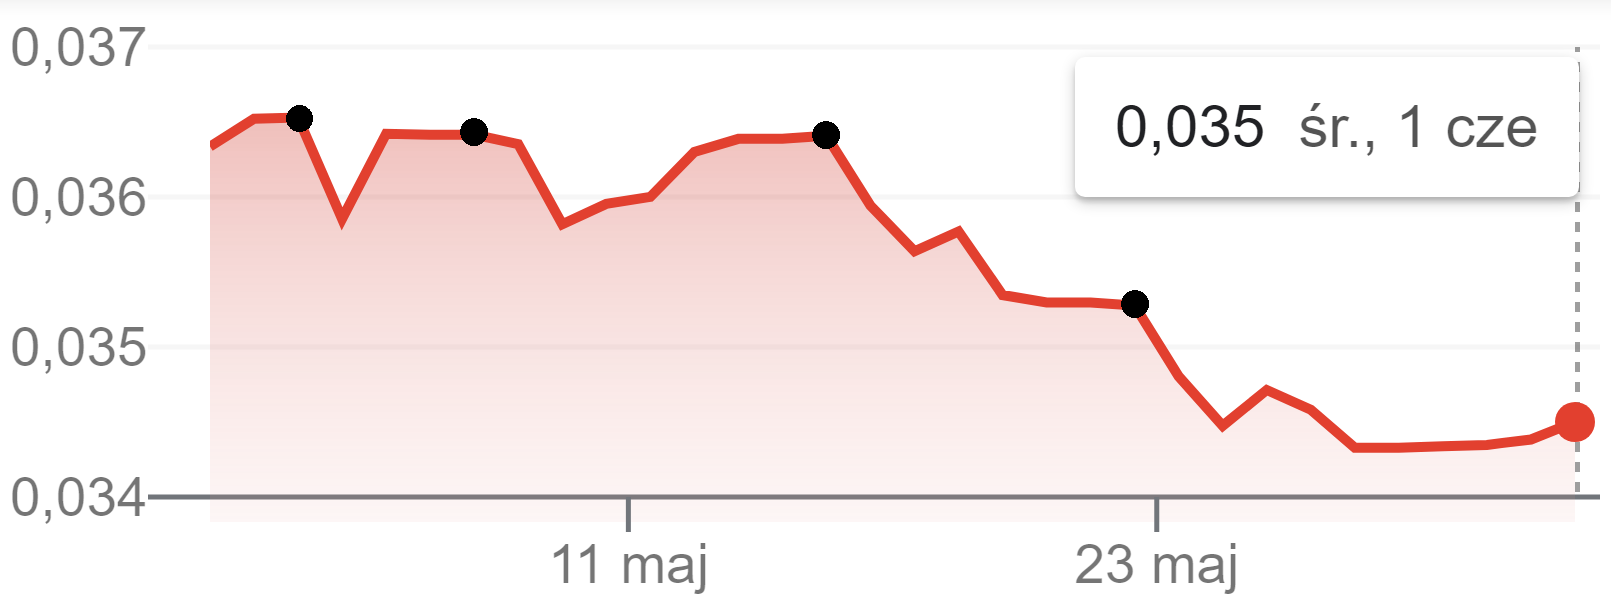
\includegraphics[height=6cm, width=\linewidth]{kurs rupii nepalskiej.png}
		\caption{Kurs rupii nepalskiej z podziałem na sekcje} \label{kurs}
	\end{center}
	\end{figure}
	
	
	
	\section{Rozwiązanie}
	\subsection{Wstęp}
	\noindent Do stworzenia sygnału wykorzystamy bloki:
	
	\begin{center}

	\begin{minipage}{0.14\linewidth}
		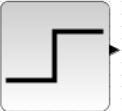
\includegraphics[width=\linewidth]{STEP_FUNCTION.png}
		\captionof*{figure}{\scriptsize STEP\textunderscore FUNCTION}
	\end{minipage}
	\hfill
	\begin{minipage}{0.15\linewidth}
		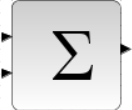
\includegraphics[width=\linewidth]{BIGSOM_f.png}
		\captionof*{figure}{\scriptsize BIGSOM\textunderscore f}
	\end{minipage}
	\hfill
	\begin{minipage}{0.15\linewidth}
		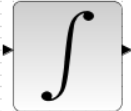
\includegraphics[width=\linewidth]{INTEGRAL_m.png}
		\captionof*{figure}{\scriptsize INTEGRAL\textunderscore m}
	\end{minipage}
	
	
	\begin{minipage}{0.15\linewidth}
		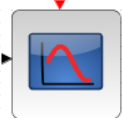
\includegraphics[width=\linewidth]{CSCOPE.png}
		\captionof*{figure}{\scriptsize CSCOPE}
	\end{minipage}
	\hfill
	\begin{minipage}{0.15\linewidth}
		
\includegraphics[width=\linewidth]{CLOCK_c.png}
		\captionof*{figure}{\scriptsize CLOCK\textunderscore c}
	\end{minipage}
	\hfill
	\begin{minipage}{0.14\linewidth}
		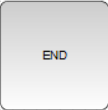
\includegraphics[width=\linewidth]{ENDBLK.png}
		\captionof*{figure}{\scriptsize ENDBLK} 
	\end{minipage}
	
	\captionof{figure}{Potrzebne bloki} \label{bloki}
	
	\end{center} 
	
	\noindent Każdy blok ma swoje parametry, które możemy modyfikować. W tym celu należy dwukrotnie nacisnąć na wybraną ikonę. W tej pracy niezbędna będzie zmiana tylko kilku z nich. Najpierw zajmijmy się elementem STEP\textunderscore FUNCTION. Parametr \textit{step time} jest czasem, w którym występuje skok Heaviside'a, a \textit{final value} oznacza jego wysokość. Sygnał, który generujemy wyświetla się dzięki oscyloskopowi CSCOPE. Jego zakres jest domyślnie ustawiony na przedział $(0;30)$, co okaże się niewystarczające przy tak złożonym sygnale jak w  sekcji Zadanie. Musimy dokonać zmian w dwóch miejscach:
	\begin{enumerate}
		\item Parametr \textit{refresh period} w oscyloskopie,
		\item Symulacja -\textgreater Ustawienia -\textgreater Ostateczny czas integracji. \\
	\end{enumerate} 
	\noindent Teraz przejdźmy do modyfikacji czysto wizualnych. Aby otrzymać dokładniej wygenerowaną funkcję powinniśmy zwiększyć taktowanie zegara, czyli zmniejszyć jego okres. Miejmy na uwadze to, że komputer będzie wykonywał wtedy więcej obliczeń, przez co czas symulacji prawdopodobnie się wydłuży. Możemy również zmienić kolor każdego z powyższych bloków (Rysunek \ref{bloki}). W tym celu należy kliknąć prawym przyciskiem myszy na wybraną ikonę, a następnie Format -\textgreater  Edycja -\textgreater  Block background. Zwiększa to przejrzystość schematu i może ułatwić referencję do konkretnej części sygnału.
	
	
	\subsection{Analiza wykresu}	
	\noindent Zauważmy, że na wykresie występują charakterystyczne okresy, gdzie rupia nepalska była stabilną walutą wobec polskiego złotego. W celu zwiększenia przejrzystości schematu w programie Xcos, podzielmy nasz sygnał wobec tego kryterium (Rysunek \ref{kurs}). Każde wypłaszczenie funkcji będzie oddzielać od siebie kolejne bloki sum.
	
	\begin{figure}[H]
		\begin{center}
			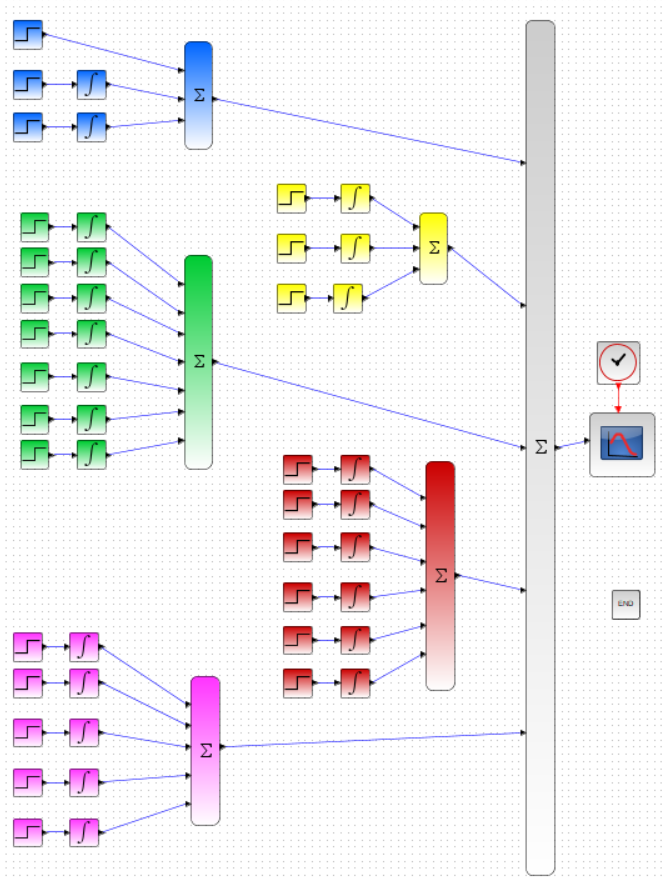
\includegraphics[scale=1]{schemat.png}
			\caption{Schemat sygnału w programie Xcos}
		\end{center}
	\end{figure}
	
	
	\subsection{Grupa niebieska}
	\noindent Pierwszy krok odpowiada za wartość początkową sygnału, dlatego ustawiamy jego czas na $0$. Zauważmy, że następny blok jest scałkowany. Interpretacją geometryczną tej operacji jest liczenie pola pod wykresem skoku Heaviside'a, dlatego otrzymamy linię prostą. Parametr \textit{final value} jest odpowiedzialny za kąt nachylenia prostej do osi $OX$. W zadaniu nie podano konkretnych wartości liczbowych, więc dobieramy go wobec uznania, tak aby zachować kształt docelowego wykresu. Przyjmijmy, że jest on równy $0.0001$. Kolejny step służy wypłaszczeniu sygnału. W tym celu ustawiamy jego parametr \textit{final value} na liczbę przeciwną do tej w poprzednim kroku (tj. $-0.0001$). W efekcie otrzymujemy sygnał równoległy do osi $OX$.
	
	\subsection{Grupa żółta}
	\noindent W tej części sygnału trzeba wykonać "ostry ząbek" w dół, więc każdy krok należy scałkować, a parametr pierwszego z nich musi być ujemny. Następnie chcemy, by sygnał odbił w górę. Dlatego \textit{final value} drugiego bloku musi być większe co do wartości bezwzględnej.	Wybrane liczby mają wpływ na kąt nachylenia wykresu do osi $OX$. Weźmy odpowiednio $-0.0004$ i $0.0007$. Trzeci krok ma na celu wyprostowanie sygnału. Jego parametr przyjmuje wartość $-0.0003$, tak aby wyzerować sumę wszystkich \textit{final values} w grupie żółtej.
	
	
	\subsection{Grupa zielona}
	\noindent Ta grupa kolorystyczna zawiera odcinki nachylone pod różnymi kątami do osi $OX$, więc każdy krok musi zostać scałkowany. Istotne jest, by dobrać \textit{final values} w taki sposób, by zachować kształt docelowego sygnału. Prościej mówiąc, musimy zwrócić szczególną uwagę jak mają się do siebie parametry sąsiadujących bloków. Zauważmy, że kierunek prostej w danym momencie czasu jest determinowany przez sumę \textit{final values} kroków, które już wystąpiły w grupie zielonej. Przyjmijmy parametry równe: 
	
	\begin{table}[H]
    \centering
    \resizebox{\textwidth}{!}{
    \begin{tblr}{|Q[c]|Q[c]|Q[c]|Q[c]|Q[c]|}
    \hline
        Numer kroku & Step time & Final value & Suma final values & Kierunek sygnału  \\ \hline
        1 & 11 & -0,00010 & -0,00010 & w dół \\ \hline
        2 & 12 & -0,00040 & -0,00050 & w dół \\ \hline
        3 & 13 & 0,00067 & 0,00017 & w górę \\ \hline
        4 & 14 & -0,00013 & 0,00004 & w górę \\ \hline
        5 & 15 & 0,00025 & 0,00029  & w górę\\ \hline
        6 & 16 & -0,00025 & 0,00004  & w górę\\ \hline
        7 & 17 & -0,00004 & 0  & sygnał wyrównany\\ \hline
    \end{tblr}
    }
	\end{table}



	\subsection{Grupa czerwona}
	\noindent Ta część sygnału jest generowana analogicznie do grupy zielonej. Zauważmy, że w 22 i 24 sekundzie sumy \textit{final values} oscylują wokół zera. Te momenty odzwierciedlają drobne fluktuacje kursu rupii nepalskiej. Z kolei w 21 sekundzie parametr bloku wynosi zaledwie $0.0001$. Choć wizualnie nie powoduje to dużej różnicy, ten krok jest odpowiedzialny za spowolnienie spadku naszej funkcji. Ostatni blok w tej grupie służy do ponownego wyrównania sygnału. Przyjmijmy parametry równe:
	
	\begin{table}[H]
    \centering
    \resizebox{\textwidth}{!}{
    \begin{tblr}{|Q[c]|Q[c]|Q[c]|Q[c]|Q[c]|}
    \hline
        Numer kroku & Step time & Final value & Suma final values  & Kierunek sygnału  \\ \hline
        1 & 20 & -0,00040 & -0,00040 & w dół  \\ \hline
        2 & 21 & 0,00010 & -0,00030 & w dół  \\ \hline
        3 & 22 & 0,00040 & 0,00010 & w górę  \\ \hline
        4 & 23 & -0,00045 & -0,00035 & w dół  \\ \hline
        5 & 24 & 0,00030 & -0,00005 & w dół  \\ \hline
        6 & 25 & 0,00005 & 0 & sygnał wyrównany  \\ \hline
    \end{tblr}
    }
	\end{table}
	
	
	
	\subsection{Grupa różowa}
	\noindent Koniec sygnału generowany jest analogicznie do poprzednich grup kolorystycznych. Każdy z kroków jest całkowany, a \textit{final values} odpowiadają za kąt nachylenia prostych do osi $OX$. Ostatni blok standardowo zeruje sumę \textit{final values}, a tym samym wyrównuje sygnał. Przyjmijmy parametry równe:
	
	
	\begin{table}[H]
    \centering
    \resizebox{\textwidth}{!}{
    \begin{tblr}{|Q[c]|Q[c]|Q[c]|Q[c]|Q[c]|}
    \hline
        Numer kroku & Step time & Final value & Suma final values  & Kierunek sygnału  \\ \hline
        1 & 27 & -0,00050 & -0,00050 & w dół  \\ \hline
        2 & 28 & 0,00020 & -0,00030 & w dół  \\ \hline
        3 & 29 & 0,00050 & 0,00020 & w górę  \\ \hline
        4 & 30 & -0,00030 & -0,00010 & w dół  \\ \hline
        5 & 32 & 0,00010 & 0,00000 & sygnał wyrównany  \\ \hline
    \end{tblr}
    }
	\end{table}
	
	
	
	\section{Wynik końcowy}
	
	\begin{figure}[H]
	\begin{center}
		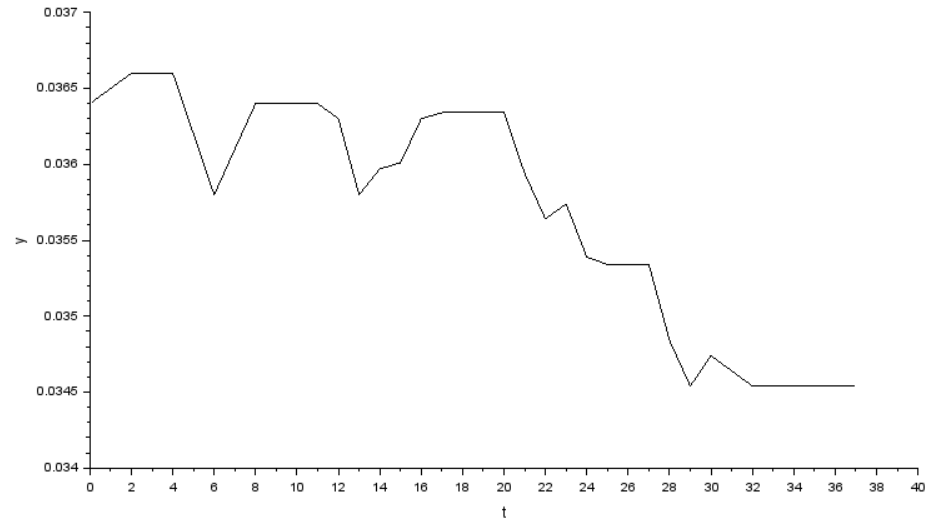
\includegraphics[width=\linewidth]{wygenerowany sygnal.png}
		\caption{Wygenerowany sygnał}
	\end{center}
	\end{figure}
	
	

\end{document}
